\section{Result analysis}
\label{sec:res}

\textit{Convert} is the function tested in the case study analysed in this report: three fuzzer instances are ran (one \textit{master} instance and two \textit{secondary} instances) and the minimised test cases corpus previously described (i.e., the minimised \textit{afl\_testcases/png/full/convert\_min} corpus) is used.

The results carried out from the fuzzing process are quantitatively collected in table \ref{tab:convert_results} and discussed below.

%Number of files used o Number of mutations generated
%– Time needed
%– Number of flaws found
%– Are the flaws found known CVEs?
\begin{table}[H]
    \centering
    \begin{tabular}{|c|c|c|c|c|}
        \hline
        \cellcolor{lightgray}\textsc{Fuzzer instance} & \cellcolor{lightgray}\textsc{\# Files used} & \cellcolor{lightgray}\textsc{\# Mutations generated} & \cellcolor{lightgray}\textsc{Time needed} & \cellcolor{lightgray}\textsc{\# Crashes found} \\
        \hline
        \textit{convert\_master} (M) & 6 & 6438 & $\simeq$ 3days & 715 (36 \textit{unique})\\
        \hline
        \textit{convert\_slave1} (S) & 6 & 7151 & $\simeq$ 3days & 6753 (396 \textit{unique}) \\
        \hline
        \textit{convert\_slave2} (S) & 6 & 7114 & $\simeq$ 3days & 6590 (386 \textit{unique}) \\
        \hline
        TOTAL & 6 & 20703 & $\simeq$ 3days & 14058 (818 \textit{unique}) \\
        \hline
    \end{tabular}
    \caption{overall results}
    \label{tab:convert_results}
\end{table}

Here follow some graphs representing the execution trend of the three fuzzer instances ran.

\begin{figure}[H]
    \centering
    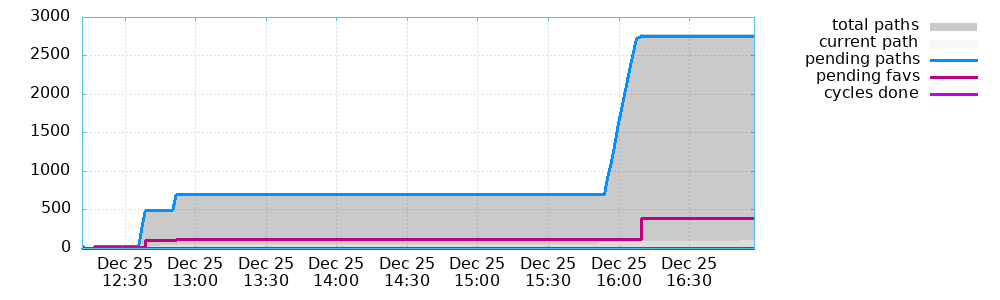
\includegraphics[width=0.5\textwidth]{Resources/convert_master/high_freq.png}\hfill
    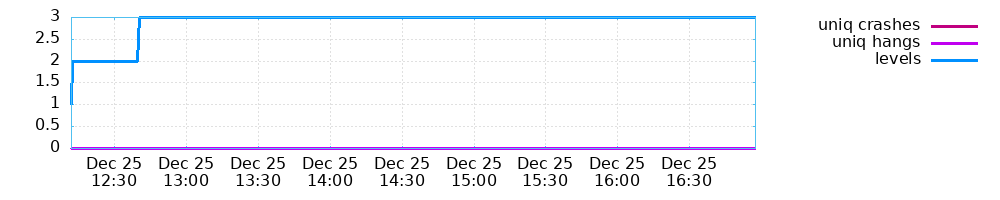
\includegraphics[width=0.5\textwidth]{Resources/convert_master/low_freq.png}
    \caption{execution trend of the \textit{master} instance \textit{convert\_master} for the first 4 hours of processing}
    \label{fig:convert_master}
\end{figure}

\begin{figure}[H]
    \centering
    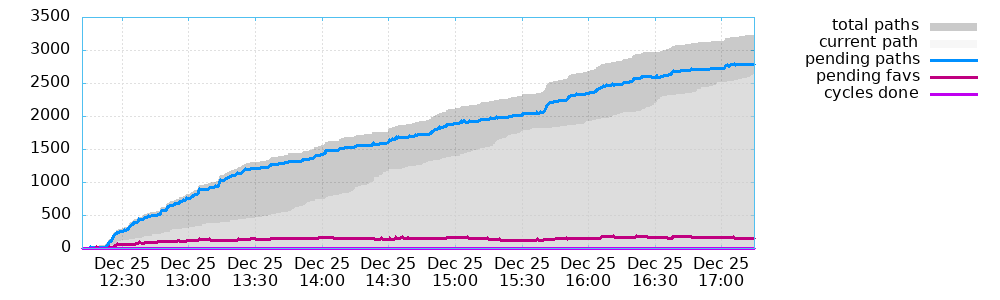
\includegraphics[width=0.5\textwidth]{Resources/convert_slave1/high_freq.png}\hfill
    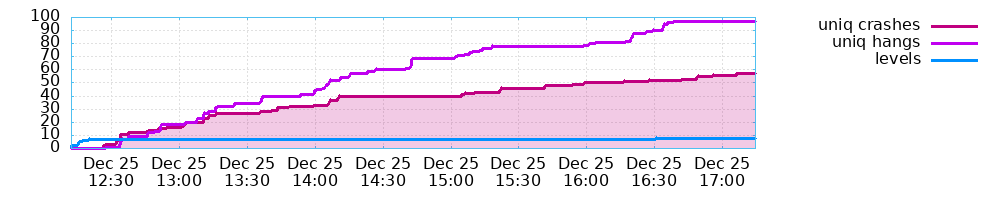
\includegraphics[width=0.5\textwidth]{Resources/convert_slave1/low_freq.png}
    \caption{execution trend of the first \textit{secondary} instance \textit{convert\_slave1} for the first 4$\frac{1}{2}$ hours of processing}
    \label{fig:convert_slave1}
\end{figure}

\begin{figure}[H]
    \centering
    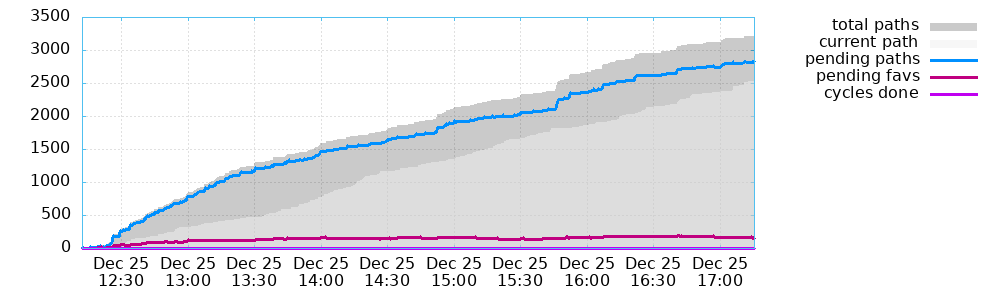
\includegraphics[width=0.5\textwidth]{Resources/convert_slave2/high_freq.png}\hfill
    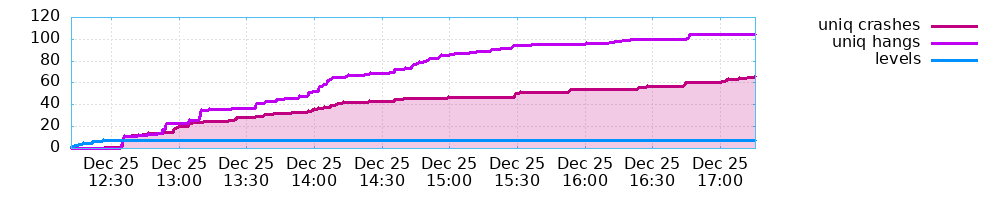
\includegraphics[width=0.5\textwidth]{Resources/convert_slave2/low_freq.png}
    \caption{execution trend of the second \textit{secondary} instance \textit{convert\_slave2} for the first 4$\frac{1}{2}$ hours of processing}
    \label{fig:convert_slave2}
\end{figure}

\subsection{Dynamic result analysis}
The crashes identified by the fuzzing process are grouped by the received signal, for instance\parencite{signals}:
\begin{description}[itemsep=0.5pt]
    \item[sig$\cdot$11]: \textit{SIGSEV} (i.e., invalid memory access - segmentation fault);
    \item[sig$\cdot$07]: \textit{SIGBUS} (i.e., bus error);
    \item[sig$\cdot$06]: \textit{SIGABRT} (i.e., abnormal termination condition).
\end{description}

Moreover, the file names for crashes and hangs are correlated with parent, non-faulting queue images\parencite{AFL_readme}: thus, a file named as "id$\cdot$000000,sig$\cdot$06,src$\cdot$000001,op$\cdot$splice,rep$\cdot$128" identifies a crash, having "000000" as identifier, correlated with the parent image whose identifier is "000001", obtained through the \textit{splice} operation (with 128 bits-rep), that causes a \textit{SIGABRT} signal.

Finally, \textit{Valgrind}\parencite{Valgrind} (actually, the \textit{Memcheck} memory error detector\parencite{MC}) is used to better analyse the crashes detected, as follows.
\begin{lstlisting}
$ valgrind <tested_program> [...]
\end{lstlisting}

\textit{Memcheck} issues a range of error messages:
\begin{itemize}
    \item illegal read / illegal write errors\parencite{MC_badrw} $\xrightarrow{}$ Invalid read of size \omissis (Address \omissis is not stack'd, malloc'd or (recently) free'd);
    \item use of uninitialised values\parencite{MC_uninitvals} $\xrightarrow{}$ Conditional jump or move depends on uninitialised value(s);
    \item use of uninitialised or unaddressable values in system calls\parencite{MC_bad-syscalls-args} $\xrightarrow{}$ Syscall param write(buf) points to uninitialised byte(s) (Address \omissis is \omissis bytes inside a block of size \omissis alloc'd);
    \item illegal frees\parencite{MC_badfrees} $\xrightarrow{}$ Invalid free() (Address \omissis is \omissis bytes inside a block of size \omissis free'd);
    \item when a heap block is freed with an inappropriate deallocation function\parencite{MC_rudefn} $\xrightarrow{}$ Mismatched free() / delete / delete [] ( Address \omissis is \omissis bytes inside a block of size \omissis alloc'd);
    \item overlapping source and destination blocks\parencite{MC_overlap} $\xrightarrow{}$ Source and destination overlap in memcpy( \omissis );
    \item fishy argument values\parencite{MC_fishyvalue} $\xrightarrow{}$ Argument 'size' of function malloc has a fishy (possibly negative) value: \omissis.
\end{itemize}

For the sake of brevity, just a small subset of the crashes collected by the fuzzer instances is analysed: one file for each $\langle sig, op \rangle$\slash $\langle sig, op, rep \rangle$ tuple and one file for each $\langle sig, op, rep \rangle$ tuple, w.r.t. the master instance and the secondary instances, respectively.
Furthermore, memory leaks\parencite{MC_leaks} are not considered in this report, for the same reason.

\subsubsection{\textit{Master} instance: \textit{convert\_master}}
\begin{description}[itemsep=0.5pt]
    %crashes_4 - id$\cdot$000004
    \item[sig$\cdot$11,src$\cdot$000370,op$\cdot$havoc,rep$\cdot$2] $\xrightarrow{}$ Invalid read of size \omissis (Address \omissis is not stack'd, malloc'd or (recently) free'd).
    
    %crashes_4 - id$\cdot$000006
    \item[sig$\cdot$11,src$\cdot$000375,op$\cdot$havoc,rep$\cdot$4] $\xrightarrow{}$ Syscall param unlink(pathname) points to unaddressable byte(s) (Address \omissis is \omissis bytes inside a block of size \omissis free'd; Block was alloc'd at \omissis); convert: unable to extend cache \omissis: File too large @ \omissis.
    
    %crashes_4 - id$\cdot$000007
    \item[sig$\cdot$11,src$\cdot$000375,op$\cdot$havoc,rep$\cdot$8] $\xrightarrow{}$ Invalid read of size \omissis (Address \omissis is not stack'd, malloc'd or (recently) free'd).
        
    %crashes_4 - id$\cdot$000027
    \item[sig$\cdot$11,src$\cdot$000791,op$\cdot$havoc,rep$\cdot$16] $\xrightarrow{}$ Killed.

    %crashes_4 - id$\cdot$000026
    \item[sig$\cdot$11,src$\cdot$000791,op$\cdot$havoc,rep$\cdot$32] $\xrightarrow{}$ Invalid read of size \omissis (Address \omissis is not stack'd, malloc'd or (recently) free'd).
    
    %crashes_4 - id$\cdot$000013
    \item[sig$\cdot$11,src$\cdot$000462,op$\cdot$havoc,rep$\cdot$64] $\xrightarrow{}$ Killed.
    
    %crashes_4 - id$\cdot$000014
    \item[sig$\cdot$11,src$\cdot$000474,op$\cdot$havoc,rep$\cdot$128] $\xrightarrow{}$ Invalid read of size \omissis (Address \omissis is not stack'd, malloc'd or (recently) free'd).
    
    %crashes_4 - id$\cdot$000016
    \item[sig$\cdot$11,src$\cdot$000613,op$\cdot$flip1,pos$\cdot$35]  $\xrightarrow{}$ convert: Unexpected end-of-file \omissis @ \omissis.
    
    %crashes_4 - id$\cdot$000000
    \item[sig$\cdot$11,src$\cdot$000368,op$\cdot$flip4,pos$\cdot$6] $\xrightarrow{}$ Argument 'size' of function malloc has a fishy (possibly negative) value: \omissis; Invalid read of size \omissis (Address \omissis is not stack'd, malloc'd or (recently) free'd).
    
    %crashes_4 - id$\cdot$000001
    \item[sig$\cdot$11,src$\cdot$000368,op$\cdot$flip16,pos$\cdot$4] $\xrightarrow{}$ Invalid read of size \omissis (Address \omissis is not stack'd, malloc'd or (recently) free'd).
    
    %crashes_4 - id$\cdot$000017
    \item[sig$\cdot$11,src$\cdot$000613,op$\cdot$arith8,pos$\cdot$1,val$\cdot$+19] $\xrightarrow{}$ convert: unable to read image data \omissis @ \omissis; convert: missing an image filename \omissis @ \omissis.

    %crashes_2 - id$\cdot$000000
    \item[sig$\cdot$11,src$\cdot$000126,op$\cdot$ext\_AO,pos$\cdot$2] $\xrightarrow{}$ Invalid read of size \omissis (Address \omissis is not stack'd, malloc'd or (recently) free'd).
\end{description}

\subsubsection{\textit{Secondary} instance: \textit{convert\_slave1}}
\begin{description}[itemsep=0.5pt]            
    %crashes_1 - id$\cdot$000011
    \item[sig$\cdot$11,src$\cdot$000151+000416,op$\cdot$splice,rep$\cdot$2] $\xrightarrow{}$ Argument 'size' of function malloc has a fishy (possibly negative) value: \omissis; Invalid read of size \omissis (Address \omissis is not stack'd, malloc'd or (recently) free'd).
    
    %crashes_1 - id$\cdot$000048
    \item[sig$\cdot$11,src$\cdot$001868+001627,op$\cdot$splice,rep$\cdot$4] $\xrightarrow{}$ Invalid read of size \omissis (Address \omissis is not stack'd, malloc'd or (recently) free'd).
    
    %crashes_1 - id$\cdot$000000
    \item[sig$\cdot$11,src$\cdot$000041+000090,op$\cdot$splice,rep$\cdot$8] $\xrightarrow{}$ Argument 'size' of function malloc has a fishy (possibly negative) value: \omissis; Invalid read of size \omissis (Address \omissis is not stack'd, malloc'd or (recently) free'd).

    %crashes_1 - id$\cdot$000001
    \item[sig$\cdot$11,src$\cdot$000041+000111,op$\cdot$splice,rep$\cdot$16] $\xrightarrow{}$ Invalid read of size \omissis (Address \omissis is not stack'd, malloc'd or (recently) free'd).
      
    %crashes_1 - id$\cdot$000025
    \item[sig$\cdot$11,src$\cdot$000390+000779,op$\cdot$splice,rep$\cdot$32] $\xrightarrow{}$ Invalid read of size \omissis (Address \omissis is not stack'd, malloc'd or (recently) free'd).
        
    %crashes_2 - id$\cdot$000030
    \item[sig$\cdot$11,src$\cdot$000539+001030,op$\cdot$splice,rep$\cdot$64] $\xrightarrow{}$ Argument 'size' of function malloc has a fishy (possibly negative) value: \omissis; Invalid read of size \omissis (Address \omissis is not stack'd, malloc'd or (recently) free'd).
    
    %crashes_1 - id$\cdot$000029
    \item[sig$\cdot$11,src$\cdot$000539+001030,op$\cdot$splice,rep$\cdot$128] $\xrightarrow{}$ Invalid read of size \omissis (Address \omissis is not stack'd, malloc'd or (recently) free'd).

    %crashes_1 - id$\cdot$000003
    \item[sig$\cdot$11,src$\cdot$000127,op$\cdot$havoc,rep$\cdot$2] $\xrightarrow{}$ Invalid read of size \omissis (Address \omissis is not stack'd, malloc'd or (recently) free'd).

    %crashes_1 - id$\cdot$000007
    \item[sig$\cdot$11,src$\cdot$000129,op$\cdot$havoc,rep$\cdot$4] $\xrightarrow{}$ Invalid read of size \omissis (Address \omissis is not stack'd, malloc'd or (recently) free'd).
    %crashes_1 - id$\cdot$000005
    \item[sig$\cdot$11,src$\cdot$000127,op$\cdot$havoc,rep$\cdot$8] $\xrightarrow{}$ Invalid read of size \omissis (Address \omissis is not stack'd, malloc'd or (recently) free'd). 
    
    %crashes_1 - id$\cdot$000004
    \item[sig$\cdot$11,src$\cdot$000127,op$\cdot$havoc,rep$\cdot$16] $\xrightarrow{}$ Argument 'size' of function malloc has a fishy (possibly negative) value: \omissis; Invalid read of size \omissis (Address \omissis is not stack'd, malloc'd or (recently) free'd).
            
    %crashes_1 - id$\cdot$000014
    \item[sig$\cdot$11,src$\cdot$000242,op$\cdot$havoc,rep$\cdot$32] $\xrightarrow{}$ Invalid read of size \omissis (Address \omissis is not stack'd, malloc'd or (recently) free'd).

    %crashes_1 - id$\cdot$000012
    \item[sig$\cdot$11,src$\cdot$000212,op$\cdot$havoc,rep$\cdot$64] $\xrightarrow{}$ Invalid read of size \omissis (Address \omissis is not stack'd, malloc'd or (recently) free'd).

    %crashes_1 - id$\cdot$000015
    \item[sig$\cdot$11,src$\cdot$000291,op$\cdot$havoc,rep$\cdot$128] $\xrightarrow{}$ Argument 'size' of function malloc has a fishy (possibly negative) value: \omissis; Invalid read of size \omissis (Address \omissis is not stack'd, malloc'd or (recently) free'd).


    %crashes_2 - id$\cdot$000006
    \item[sig$\cdot$06,src$\cdot$002637+003167,op$\cdot$splice,rep$\cdot$2] $\xrightarrow{}$ Conditional jump or move depends on uninitialised value(s)\footnotemark[1]; Syscall param write(buf) points to uninitialised byte(s) (Address \omissis is \omissis bytes inside a block of size \omissis alloc'd)\footnotemark[1]; convert: Unexpected end-of-file \omissis: No such file or directory @ \omissis.
    
    %crashes_1 - id$\cdot$000055
    \item[sig$\cdot$06,src$\cdot$002457+002963,op$\cdot$splice,rep$\cdot$4] $\xrightarrow{}$ convert: Unexpected end-of-file \omissis: No such file or directory @ \omissis.
        
    %crashes_2 - id$\cdot$000005
    \item[sig$\cdot$06,src$\cdot$002637+003167,op$\cdot$splice,rep$\cdot$8] $\xrightarrow{}$ Conditional jump or move depends on uninitialised value(s)\footnotemark[1]; Syscall param write(buf) points to uninitialised byte(s) (Address \omissis is \omissis bytes inside a block of size \omissis alloc'd)\footnotemark[1].
        
    %crashes_1 - id$\cdot$000053
    \item[sig$\cdot$06,src$\cdot$002361+002347,op$\cdot$splice,rep$\cdot$16] $\xrightarrow{}$ convert: Unexpected end-of-file \omissis: No such file or directory @ \omissis.
    
    %crashes_2 - id$\cdot$000004
    \item[sig$\cdot$06,src$\cdot$002637+003167,op$\cdot$splice,rep$\cdot$32] $\xrightarrow{}$ Conditional jump or move depends on uninitialised value(s)\footnotemark[1]; Syscall param write(buf) points to uninitialised byte(s) (Address \omissis is \omissis bytes inside a block of size \omissis alloc'd)\footnotemark[1]; convert: Unexpected end-of-file \omissis: No such file or directory @ \omissis.

    %crashes_1 - id$\cdot$000056
    \item[sig$\cdot$06,src$\cdot$002541+000333,op$\cdot$splice,rep$\cdot$64] $\xrightarrow{}$ convert: Unexpected end-of-file \omissis: No such file or directory @ \omissis.

    %crashes_4 - id$\cdot$000020
    \item[sig$\cdot$06,src$\cdot$005324+003962,op$\cdot$splice,rep$\cdot$128] $\xrightarrow{}$ convert: Unexpected end-of-file \omissis: No such file or directory @ \omissis.

    %crashes_3 - id$\cdot$000050
    \item[sig$\cdot$06,src$\cdot$003816,op$\cdot$havoc,rep$\cdot$4] $\xrightarrow{}$ convert: Unexpected end-of-file \omissis: No such file or directory @ \omissis.
    
    %crashes_1 - id$\cdot$000054
    \item[sig$\cdot$06,src$\cdot$002413,op$\cdot$havoc,rep$\cdot$8] $\xrightarrow{}$ convert: Unexpected end-of-file \omissis: No such file or directory @ \omissis.
        
    %crashes_2 - id$\cdot$000015
    \item[sig$\cdot$06,src$\cdot$003132,op$\cdot$havoc,rep$\cdot$16] $\xrightarrow{}$ convert: Unexpected end-of-file \omissis: No such file or directory @ \omissis. 
    
    %crashes_4 - id$\cdot$000055
    \item[sig$\cdot$06,src$\cdot$005795,op$\cdot$havoc,rep$\cdot$32] $\xrightarrow{}$ Invalid write of size \omissis (Address \omissis is \omissis bytes after a block of size \omissis alloc'd)\footnotemark[1]; Use of uninitialised value of size \omissis\footnotemark[1]; Invalid read of size \omissis (Address \omissis is \omissis bytes after a block of size \omissis alloc'd)\footnotemark[1]; Invalid read of size \omissis (Address \omissis is \omissis bytes before a block of size \omissis in arena "client")\footnotemark[1]; Syscall param write(buf) points to uninitialised byte(s) (Address \omissis is \omissis bytes inside a block of size \omissis alloc'd)\footnotemark[1]; Syscall param unlink(pathname) points to unaddressable byte(s) (Address \omissis is \omissis bytes inside a block of size \omissis free'd; Block was alloc'd at \omissis); convert: unable to extend cache \omissis: File too large @ \omissis; sh: 1: rawtorle: not found; convert: Unexpected end-of-file \omissis: No such file or directory @ \omissis. 

    %crashes_1 - id$\cdot$000052
    \item[sig$\cdot$06,src$\cdot$002332,op$\cdot$havoc,rep$\cdot$64] $\xrightarrow{}$ Conditional jump or move depends on uninitialised value(s)\footnotemark[1]; Syscall param write(buf) points to uninitialised byte(s) (Address \omissis is \omissis bytes inside a block of size \omissis alloc'd)\footnotemark[1]; convert: Unexpected end-of-file \omissis: No such file or directory @ \omissis.


     %crashes_4 - id$\cdot$000161
    \item[sig$\cdot$07,src$\cdot$006053+005307,op$\cdot$splice,rep$\cdot$32] $\xrightarrow{}$ Invalid write of size \omissis (Address \omissis is \omissis bytes after a block of size \omissis in arena "client"); valgrind: \omissis: Assertion \omissis failed; valgrind: Heap block lo/hi size mismatch: \omissis.
\end{description}

\subsubsection{\textit{Secondary} instance: \textit{convert\_slave2}}
\begin{description}[itemsep=0.5pt]
    %crashes_1 - id$\cdot$000012
    \item[sig$\cdot$11,src$\cdot$000182+000386,op$\cdot$splice,rep$\cdot$2] $\xrightarrow{}$ Invalid read of size \omissis (Address \omissis is not stack'd, malloc'd or (recently) free'd).
    
    %crashes_1 - id$\cdot$000011
    \item[sig$\cdot$11,src$\cdot$000155+000386,op$\cdot$splice,rep$\cdot$4] $\xrightarrow{}$ Invalid read of size \omissis (Address \omissis is not stack'd, malloc'd or (recently) free'd).
    
    %crashes_1 - id$\cdot$000025
    \item[sig$\cdot$11,src$\cdot$000441+001037,op$\cdot$splice,rep$\cdot$8] $\xrightarrow{}$ Argument 'size' of function malloc has a fishy (possibly negative) value: \omissis; Invalid read of size \omissis (Address \omissis is not stack'd, malloc'd or (recently) free'd).
    
    %crashes_1 - id$\cdot$000015
    \item[sig$\cdot$11,src$\cdot$000319+000435,op$\cdot$splice,rep$\cdot$16] $\xrightarrow{}$ Invalid read of size \omissis (Address \omissis is not stack'd, malloc'd or (recently) free'd).
    
    %crashes_1 - id$\cdot$000023
    \item[sig$\cdot$11,src$\cdot$000345+000602,op$\cdot$splice,rep$\cdot$32] $\xrightarrow{}$ Argument 'size' of function malloc has a fishy (possibly negative) value: \omissis; Invalid read of size \omissis (Address \omissis is not stack'd, malloc'd or (recently) free'd). 
    
    %crashes_1 - id$\cdot$000026
    \item[sig$\cdot$11,src$\cdot$000447+000886,op$\cdot$splice,rep$\cdot$64] $\xrightarrow{}$ Argument 'size' of function malloc has a fishy (possibly negative) value: \omissis; Invalid read of size \omissis (Address \omissis is not stack'd, malloc'd or (recently) free'd).
    
    %crashes_1 - id$\cdot$000014
    \item[sig$\cdot$11,src$\cdot$000246+000582,op$\cdot$splice,rep$\cdot$128] $\xrightarrow{}$ Invalid read of size \omissis (Address \omissis is not stack'd, malloc'd or (recently) free'd).

    %crashes_1 - id$\cdot$000003
    \item[sig$\cdot$11,src$\cdot$000139,op$\cdot$havoc,rep$\cdot$2] $\xrightarrow{}$ Argument 'size' of function malloc has a fishy (possibly negative) value: \omissis; Invalid read of size \omissis (Address \omissis is not stack'd, malloc'd or (recently) free'd).
        
    %crashes_1 - id$\cdot$000039
    \item[sig$\cdot$11,src$\cdot$000892,op$\cdot$havoc,rep$\cdot$4] $\xrightarrow{}$ Invalid read of size \omissis (Address \omissis is not stack'd, malloc'd or (recently) free'd).
      
    %crashes_1 - id$\cdot$000002
    \item[sig$\cdot$11,src$\cdot$000139,op$\cdot$havoc,rep$\cdot$8] $\xrightarrow{}$ Argument 'size' of function malloc has a fishy (possibly negative) value: \omissis; Invalid read of size \omissis (Address \omissis is not stack'd, malloc'd or (recently) free'd).
    
    %crashes_1 - id$\cdot$000001
    \item[sig$\cdot$11,src$\cdot$000139,op$\cdot$havoc,rep$\cdot$16] $\xrightarrow{}$ convert: unable to extend cache \omissis: File too large @ \omissis; Syscall param unlink(pathname) points to unaddressable byte(s) (Address \omissis is \omissis bytes inside a block of size \omissis free'd; Block was alloc'd at \omissis).
    
    %crashes_1 - id$\cdot$000000
    \item[sig$\cdot$11,src$\cdot$000043,op$\cdot$havoc,rep$\cdot$32] $\xrightarrow{}$ Invalid read of size \omissis (Address \omissis  is not stack'd, malloc'd or (recently) free'd).

    %crashes_1 - id$\cdot$000029
    \item[sig$\cdot$11,src$\cdot$000536,op$\cdot$havoc,rep$\cdot$64] $\xrightarrow{}$ Argument 'size' of function malloc has a fishy (possibly negative) value: \omissis; Invalid read of size \omissis (Address \omissis is not stack'd, malloc'd or (recently) free'd).
    
    %crashes_1 - id$\cdot$000041
    \item[sig$\cdot$11,src$\cdot$000926,op$\cdot$havoc,rep$\cdot$128] $\xrightarrow{}$ Invalid read of size \omissis (Address \omissis is not stack'd, malloc'd or (recently) free'd).

    
    %crashes_1 - id$\cdot$000064
    \item[sig$\cdot$06,src$\cdot$002519+002803,op$\cdot$splice,rep$\cdot$2] $\xrightarrow{}$ convert: Unexpected end-of-file \omissis: No such file or directory @ \omissis.
    
    %crashes_1 - id$\cdot$000053
    \item[sig$\cdot$06,srcv001824+002571,op$\cdot$splice,rep$\cdot$4] $\xrightarrow{}$ Conditional jump or move depends on uninitialised value(s)\footnotemark[1]; Syscall param write(buf) points to uninitialised byte(s) (Address \omissis is \omissis bytes inside a block of size \omissis alloc'd)\footnotemark[1]; convert: Unexpected end-of-file \omissis: No such file or directory @ \omissis.
    
    %crashes_2 - id$\cdot$000014
    \item[sig$\cdot$06,src$\cdot$003597+003572,op$\cdot$splice,rep$\cdot$8] $\xrightarrow{}$ Conditional jump or move depends on uninitialised value(s)\footnotemark[1]; Syscall param write(buf) points to uninitialised byte(s) (Address \omissis is \omissis bytes inside a block of size \omissis alloc'd); Use of uninitialised value of size \omissis; convert: Invalid colormap index \omissis @ \omissis.
    
    %crashes_1 - id$\cdot$000061
    \item[sig$\cdot$06,src$\cdot$002373+000953,op$\cdot$splice,rep$\cdot$16] $\xrightarrow{}$ Conditional jump or move depends on uninitialised value(s)\footnotemark[1]; Syscall param write(buf) points to uninitialised byte(s) (Address \omissis is \omissis bytes inside a block of size \omissis alloc'd); Use of uninitialised value of size \omissis; convert: Unexpected end-of-file \omissis: No such file or directory @ \omissis.
    
    %crashes_2 - id$\cdot$000053
    \item[sig$\cdot$06,src$\cdot$002368+001235,op$\cdot$splice,rep$\cdot$32] $\xrightarrow{}$ convert: Unexpected end-of-file \omissis: No such file or directory @ \omissis.

    %crashes_4 - id$\cdot$000046
    \item[sig$\cdot$06,src$\cdot$005745+003486,op$\cdot$splice,rep$\cdot$64] $\xrightarrow{}$ Invalid write of size \omissis (Address \omissis is \omissis bytes after a block of size \omissis alloc'd)\footnotemark[1]; VALGRIND INTERNAL ERROR: Valgrind received a signal 11 (SIGSEGV) - exiting \omissis; valgrind: the 'impossible' happened: Killed by fatal signal.
        
    %crashes_1 - id$\cdot$000063
    \item[sig$\cdot$06,src$\cdot$002452+001646,op$\cdot$splice,rep$\cdot$128] $\xrightarrow{}$ convert: Unexpected end-of-file \omissis: No such file or directory @ \omissis.
        
    %crashes_2 - id$\cdot$000020
    \item[sig$\cdot$06,src$\cdot$004130,op$\cdot$havoc,rep$\cdot$2] $\xrightarrow{}$ convert: Unexpected end-of-file \omissis: No such file or directory @ \omissis.
    
    %crashes_1 - id$\cdot$000065
    \item[sig$\cdot$06,src$\cdot$002536,op$\cdot$havoc,rep$\cdot$4] $\xrightarrow{}$ convert: Unexpected end-of-file \omissis: No such file or directory @ \omissis.
    
    %crashes_1 - id$\cdot$000062
    \item[sig$\cdot$06,src$\cdot$002377,op$\cdot$havoc,rep$\cdot$8] $\xrightarrow{}$ Invalid read of size \omissis (Address \omissis is \omissis bytes after a block of size \omissis alloc'd)\footnotemark[1]; convert: Unexpected end-of-file \omissis: No such file or directory @ \omissis.
    
    %crashes_2 - id$\cdot$000010
    \item[sig$\cdot$06,src$\cdot$003137,op$\cdot$havoc,rep$\cdot$16] $\xrightarrow{}$ Conditional jump or move depends on uninitialised value(s)\footnotemark[1]; Syscall param write(buf) points to uninitialised byte(s) (Address \omissis is \omissis bytes inside a block of size \omissis alloc'd); Use of uninitialised value of size \omissis; convert: Unexpected end-of-file \omissis: No such file or directory @ \omissis.
    
    %crashes_2 - id$\cdot$000011
    \item[sig$\cdot$06,src$\cdot$003137,op$\cdot$havoc,rep$\cdot$32] $\xrightarrow{}$ convert: Unexpected end-of-file \omissis: No such file or directory @ \omissis.
    
    %crashes_1 - id$\cdot$000060
    \item[sig$\cdot$06,src$\cdot$002373,op$\cdot$havoc,rep$\cdot$64] $\xrightarrow{}$ Conditional jump or move depends on uninitialised value(s)\footnotemark[1]; Syscall param write(buf) points to uninitialised byte(s) (Address \omissis is \omissis bytes inside a block of size \omissis alloc'd); Use of uninitialised value of size \omissis; convert: Unexpected end-of-file \omissis: No such file or directory @ \omissis.
\end{description}

\footnotetext[1]{\#error messages $>$ 1.}

\subsection{Bug fixing}
Since the \textit{ImageMagick} release tested has been hugely fixed, the crash-leading files previously detected do not make the most recent version of (legacy) \textit{ImageMagick} (i.e., \textit{ImageMagick-6.9.12-71}) crash: the flaws found are clearly known (removed) vulnerabilities\parencite{IM_CVE1}\parencite{IM_CVE2}\parencite{IM_CVE3}\parencite{IM_CVE4}\parencite{IM_CVE5}\parencite{IM_CVE6}\parencite{IM_CVE7}\parencite{IM_CVE8}\parencite{IM_CVE10}.